\chapter{Návrh projektu}

\section{Výběr technologií}

\subsection{Frontend}
Ačkoliv se trendy v oblasti vývoje webových aplikací mění velmi rychle,
jednou z nejpodstatnějších změn, která přenesla vykreslování stránky
na stranu uživatele a tim se výrazně odlišila od dosavadních konceptů
vykreslujících stránku na straně serveru, se stala technologie
\textbf{Single page aplication}. Celá aplikace pak je v tomto duchu
implementována a přizpůsobena s důrazem na plynulost a rychlost aplikace.

\subsubsection{Single page aplication}
Single page aplication je technologie umožnující vykreslení jiné stránky,
bez nutnosti, posílaní requestu na server.
Uživatel si při prvním spuštění webu stáhne celý balíček webu a 
při opětovném načtení vetšinou sahá jen do své lokální cache.
JavaScriptová knihovna (v tomto případě React)
poté stránku překresluje při uživatelské interakci.
V případě nutnosti stažení / posílaní dat mezi serverem a uživatelem
(např. editace záznamu, nebo načtení existujícího záznamu)
se volá pouze request k API webové služby a tělo requestu obsahuje pouze
užitečné (ne-redundantní) informace. 


\subsubsection{React}
Knihovna React poskytuje single page aplication technologii.
Jedná se o dobře udržovanou knihovnu, jež byla vyvinuta Facebookem 
jakožto náhrada zastaralého konceptu renderovaní stránky na serveru.
Díky tomu servery nemusejí ztrácet výkon s každou změnou na stránce a
výkon k renderovaní se bere z PC uživatele.
Jádro této knihovny je velmi dobře optimalizované a poskytuje i řadu
debuggovacích nástrojů, což je pro větší projekty nepostradatelná výhoda.  


\subsubsection{Další možné technologie}
Běžnou praxí vykreslování dynamické stránky je její vykreslení na straně serveru,
jako to má např. velmi populární redakční systém WordPress (jež je psaný v jazyce PHP).
Takovýto system je dobře uživatelsky přivětivý, ale za cenu masivního nárůstu
potřebného serverového výkonu.
V případě implementace knihovního systému by to znamenalo vykreslovat
celou stránku (hlavičku, tělo i zápatí) na serveru,
na druhé straně single page aplication na serveru nic nevykresluje a
pouze minimalisticky posílá požadované informace.


\subsection{Backend}
Mít single page aplikaci na frontendu znamená, že na backendu musí existovat API,
od kterého bude frontend čerpat data.
Navíc zde potřebujeme i systém pro statické odesílaní balíku celé webové stránky.
V rámci udržitelnosti byl použit stejný jazyk JavaScript, jaký je na frontendu.
Knihovnou, která by umožňovala komplexní správu requestů a zároveň by byla
i na robustnějších projektech programátorsky přehledná, byla zvolena Express.js.

\subsubsection{Express.js}
Express.js poskytuje nejen odesílaní statických stránek,
což je potřeba při odesílání balíku s aplikací React, ale umí i
custom requesty, potřebné pro rozmanité API a také odesílaní a
lokální ukládaní statických souborů, jako jsou obrázky a word nebo pdf dokumenty.

\subsubsection{MongoDB}
MongoDB je databázový systém typu non-SQL.
Což primárně znamená, že data neuchovává v tabulkách, ale v tzv. schématech.
Což má mnoho výhod, z nichž největší je, že nekompletní záznamy nezabírají
svými nevyplněnými daty místo v DB a ukládá se opravdu jen to, co je potřeba.
Další výhodou je styl ukládaní dat a komunikace s DB.
Databáze si data uchovává ve formátu BSON (binární JSON rozšířený o datové typy).
O data si aplikace žádá pomoci query,
která je zcela odlišná od těch u SQL databází,
primárně se zde neposílá query ve formátu string ale jako JSON objekt,
díky čemuž např. nenastane známá SQL injection.
Znovu ve formátu JSON poté data vrací aplikaci.

\subsubsection{Další možné technologie}
Díky odděleni frontendu a backendu (narozdíl od např. WordPressu) je možné
na backend nasadit téměř cokoliv co umí posílat requesty.
Příkladem toho můžou být scripty v jazycích PHP, C\#, Python, nebo Perl.
Ale vzhledem k tomu, že jedním z modulů bude neuronová síť na pokročilé vyhledávaní,
vybírali jsme mezi jazyky Python a JavaScript, jakožto dvěma jazyky, které
mají velmi dobré knihovny pro práci s neuronovými sítěmi.

\section{Diagram systému}
\begin{figure}[H]
	\centering
	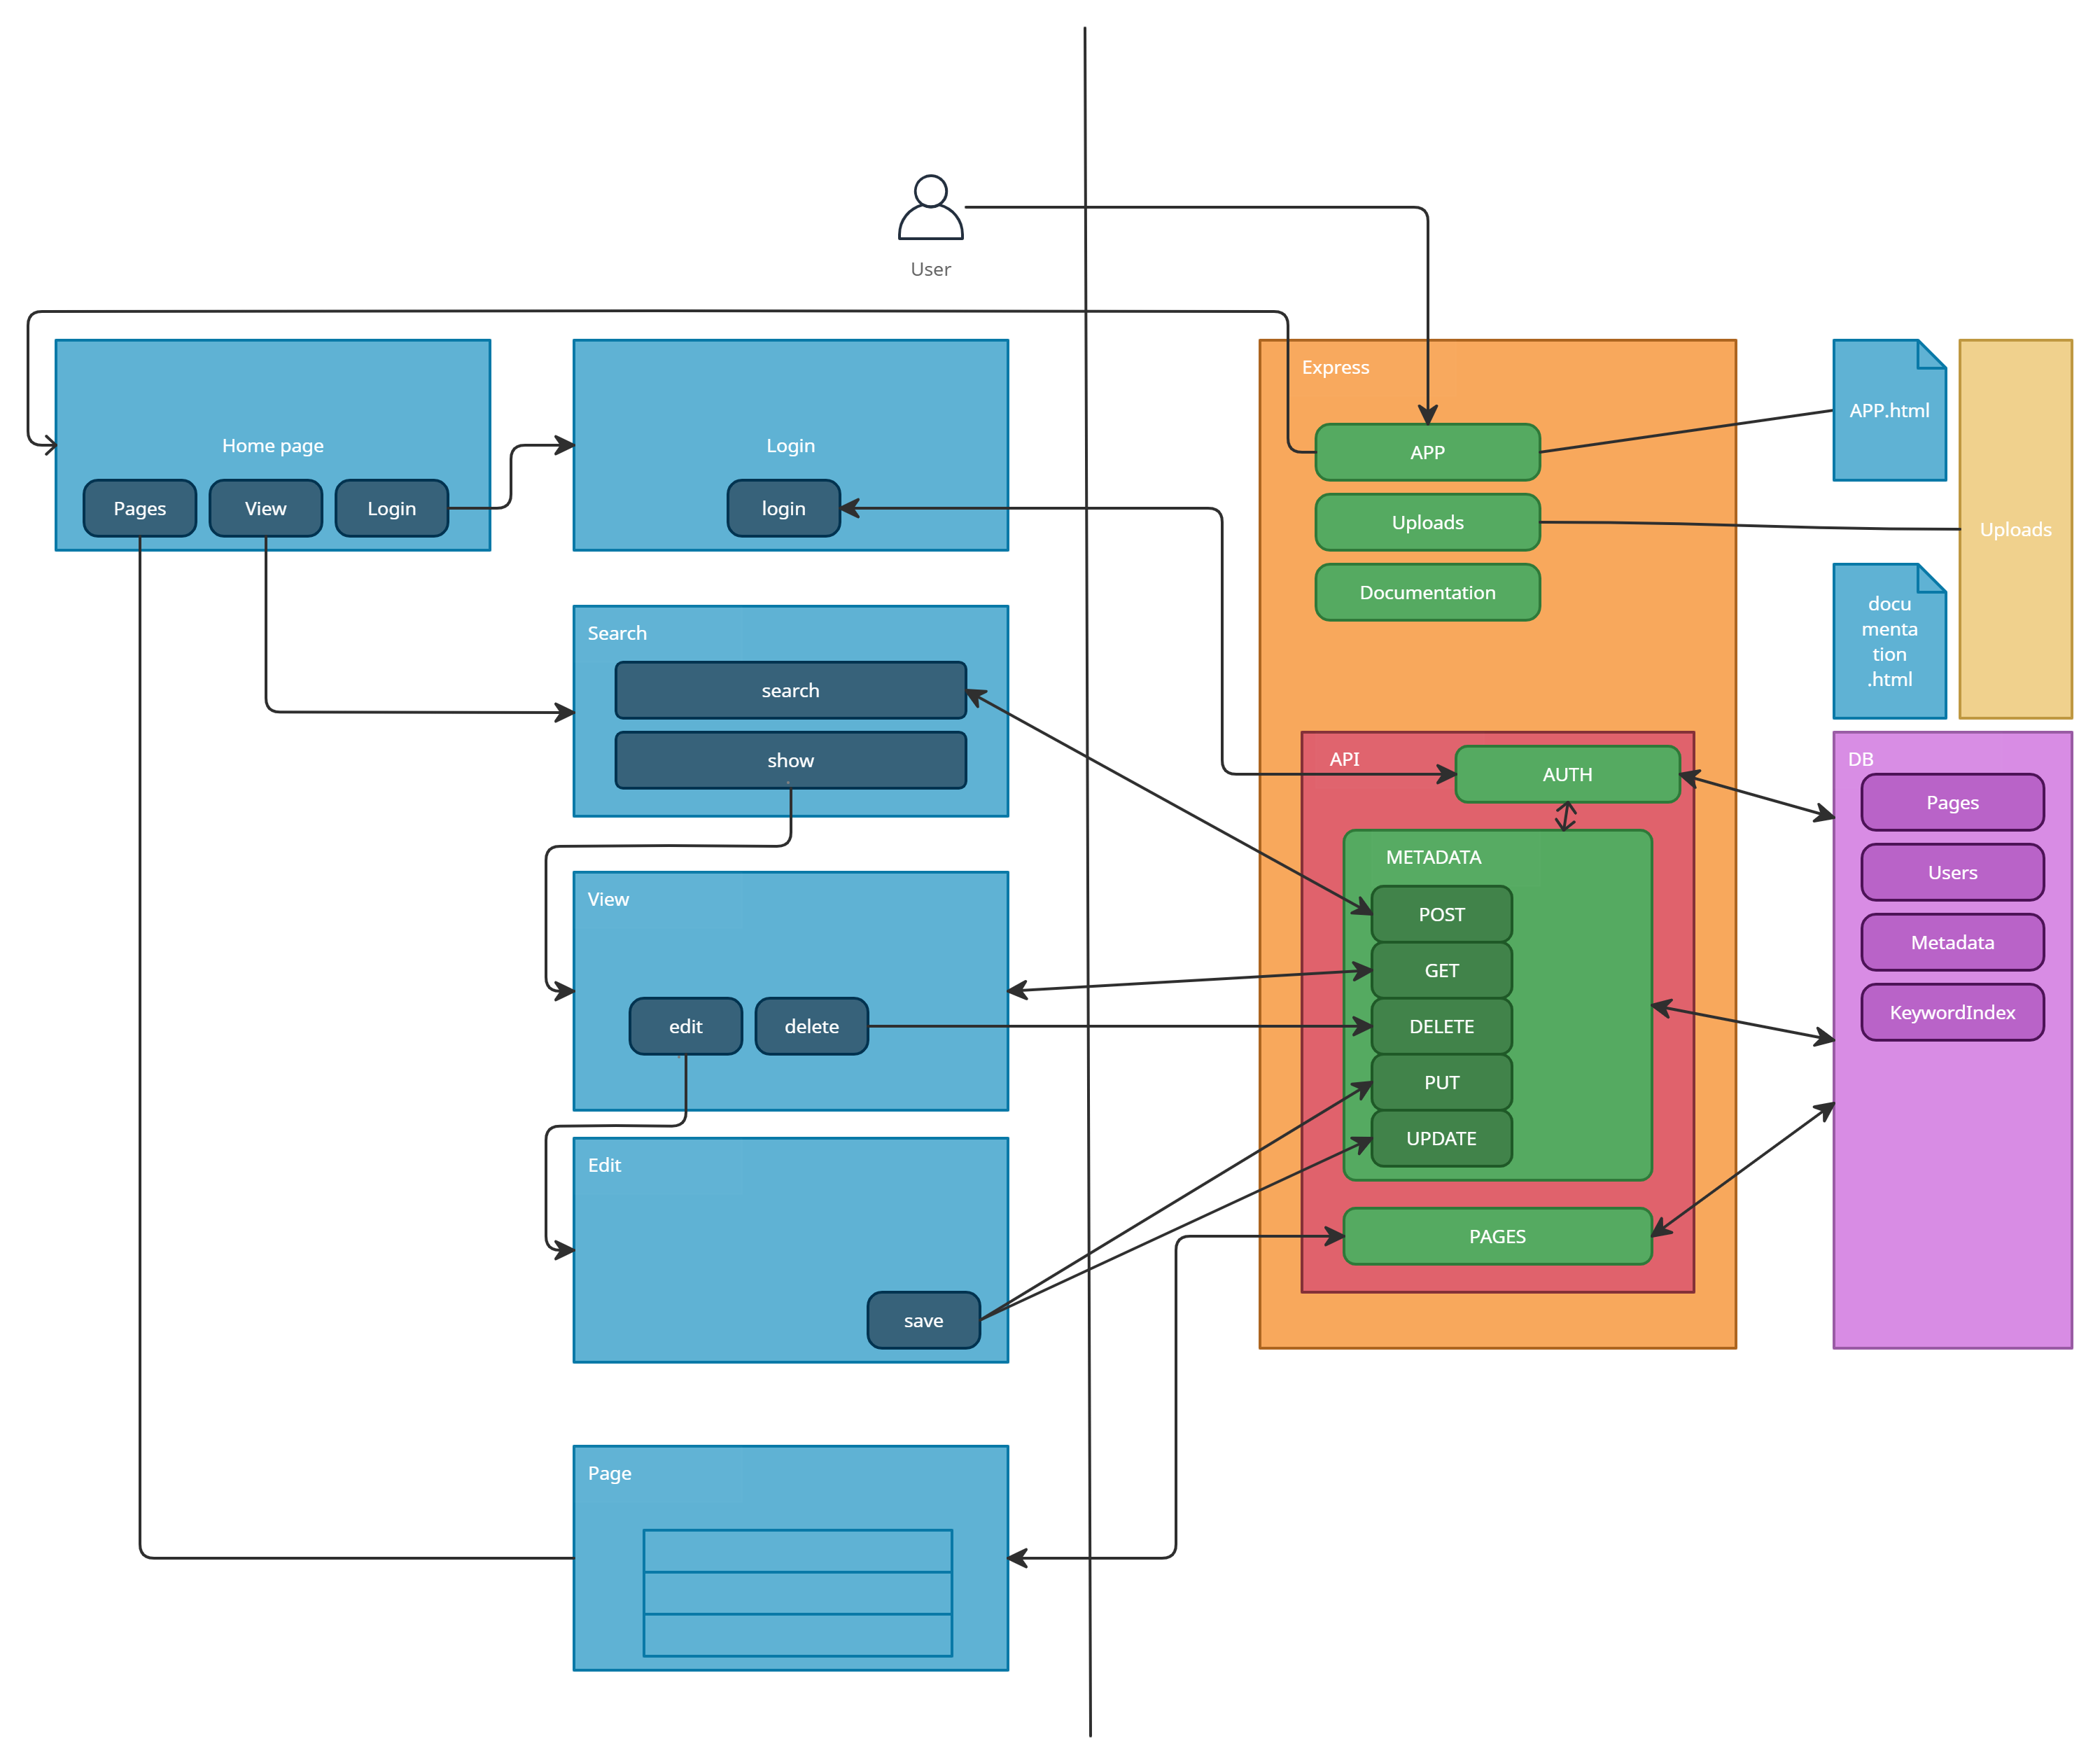
\includegraphics[angle=-90,origin=c,width=\linewidth]{img/diagram.png}
	\caption{Diagram systému}
\end{figure}
